\chapter{測定、ユニタリ発展、量子力学}

\lectureoverview{まず、すでに用いてきた測定の原理をまとめておく。すなわち、観測量はエルミート演算子であり、その固有値が可能な測定結果であり、区別可能な状態は直交し、ボルンの規則が確率を与える。新しい問題は力学である。可逆性は、重なりを保つ共通の線形発展を要求する。このことから発展演算子はユニタリとなり、その無限小生成子はエルミートとなる。生成子はハミルトニアンであり、その作用が時間依存のSchr\"odinger方程式を与える。次に期待値の公式、平均値に対する交換子方程式、古典的ポアソン括弧との関係、そして平均エネルギーの保存を導く。}

当面はスピン系を脇に置く。一般的な構造が整った後で、これに戻る。以下の原理は、最小限の独立な集合として提示されるものではない。いくつかは他のものを補強したり部分的に含意したりするが、別々に述べることでその物理的内容が見やすくなる。

\section{測定が返しうるもの}

\emph{観測量}とは、測定できるものである。定着した用語は必要以上に大げさであり、\emph{測定可能量}でも十分であっただろう。各観測量にはエルミート演算子を対応させる。当面、そのような演算子を\(L\)で表す。
\begin{equation}
L^\dagger=L.
\end{equation}
すべての線形演算子がエルミートであるわけではない。逆に、あるエルミート演算子が利用可能な材料と装置で測定できるかどうかは、難しい実験的問題でありうる。それでも抽象的な作業規則は寛容である。エルミート演算子は、実際の測定がまだ発明されていなくても、可能な観測量を表す。

もし
\begin{equation}
L\ket{\lambda}=\lambda\ket{\lambda},
\end{equation}
ならば、\(\lambda\)は\(L\)を測定したときの可能な数値結果である。固有値とその固有ベクトルを同じ記号で表す。ケットの括弧が両者を区別する。\(\lambda\)は数であり、\(\ket{\lambda}\)は状態である。

なぜエルミート演算子なのか。原始的な装置は実数を報告する。もし計器が1つの複素数を報告しているように見えるなら、実際には2つの独立な実量を報告している。したがって、観測量の固有値は実数でなければならない。さらに、異なる確定した結果に対応する状態は物理的に区別可能でなければならず、したがって直交する。ここで用いる有限次元の設定では、完全な正規直交固有基底と実固有値をもつ線形演算子はエルミートである。したがって、物理的な言明とエルミート構造は互いに整合する。

\subsection{区別可能性は直交性である}

\emph{物理的に区別可能}という語句には操作的な意味がある。スピンが上または下のいずれかに準備されるとしよう。\(z\)軸に沿った測定は、曖昧さなく可能性を分離する。上は\(+1\)を与え、下は\(-1\)を与える。同様に、左と右は\(x\)軸に沿った測定によって区別できる。

次に、準備が上または右のいずれかであるとしよう。\(z\)測定は、上に対して確実に\(+1\)を与えるが、右の状態も非零の確率で\(+1\)を与える。\(x\)測定は単に非対称性を逆にするだけである。装置を\(45^\circ\)傾けても、結果の分布の間の重なりは取り除かれない。どのような向きも、2つの準備を常に区別する結果を生み出さない。

\begin{definition}
何らかの実験、または実験の集まりが、どちらの準備が与えられたかを曖昧さなく決定できるとき、2つの状態は物理的に区別可能である。
\end{definition}

量子力学は完全な区別可能性を幾何学的に表す。
\begin{equation}
\text{distinguishable states}
\quad\Longrightarrow\quad
\text{orthogonal vectors}.
\end{equation}

\begin{classroomqa}
\audiencequestion{異なる測定軸は上状態と右状態を区別できるだろうか。}
\lecturerresponse{いいえ。\(z\)または\(x\)に沿った測定は、ときに準備を同定できるが、少なくとも1つの結果は両方と両立したままである。中間の軸も重なり合う確率を残す。障害は装置の選択が悪いことではない。2つの状態ベクトルが直交していないのである。}
\end{classroomqa}

\section{ボルンの規則}

固有値は何が起こり得るかを教えてくれるが、どれほど頻繁に起こるかは教えてくれない。確率規則が予測内容を与える。規格化された系が\(\ket{A}\)に用意され、規格化された固有ベクトル\(\ket{\lambda}\)が測定される観測量\(L\)に属するなら、
\begin{equation}
P(\lambda)=\left|\braket{\lambda}{A}\right|^2.
\label{eq:l4-born-rule}
\end{equation}
重なり\(\braket{\lambda}{A}\)は\emph{確率振幅}である。それは一般に複素数であるため、それ自体が確率になることはできない。その絶対値の二乗は実数かつ非負である。

\begin{figure}[htbp]
\centering
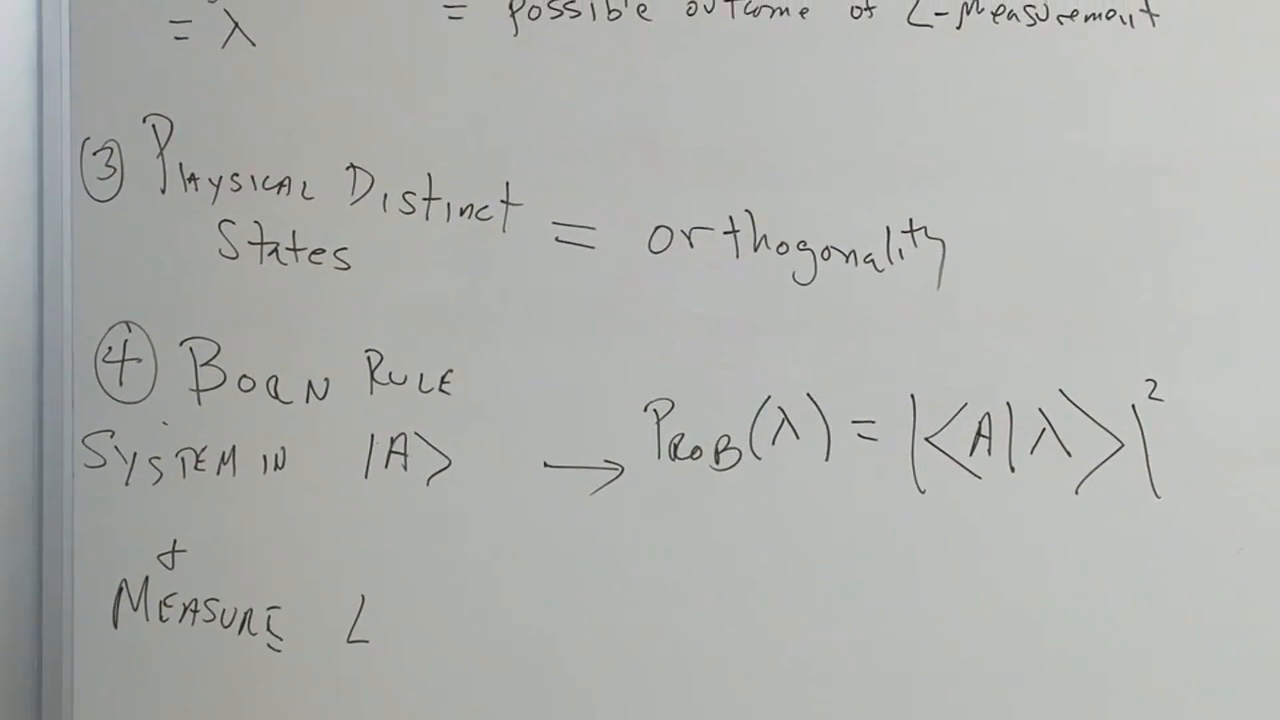
\includegraphics[width=0.86\textwidth]{lecture_04_figure_01.png}
\caption{測定原理の傍らに記されたボルンの規則：確率は重なりの絶対値の二乗である。}
\lectureframe{00:12:40}
\end{figure}

\(L\)の正規直交固有基底を選び、
\begin{equation}
\ket{A}=\sum_i \alpha_i\ket{\lambda_i},
\qquad
\alpha_i=\braket{\lambda_i}{A}.
\end{equation}
と展開する。ボルンの規則は
\begin{equation}
P(\lambda_i)=|\alpha_i|^2.
\end{equation}
となる。規格化により
\begin{equation}
\sum_i P(\lambda_i)=\sum_i|\alpha_i|^2=1.
\end{equation}
が得られる。正値性と規格化の要請だけからボルンの規則が導かれるわけではないが、絶対値の二乗がなぜこれほど自然に確率論に適合するかが示される。最終的には、この規則は実験によって検証される。

\begin{classroomqa}
\audiencequestion{絶対値の二乗は、すべての確率が1に足し合わされるためにも必要なのでしょうか。}
\lecturerresponse{正規直交基底で展開された規格化された状態に対しては、振幅の二乗は確かに1に足し合わされる。したがって、正値性と規格化はボルンの規則に完全に適合する。どちらの主張を論理的に先行すると見なすべきかはここではあまり重要ではなく、それらの相互整合性の方が重要である。確率規則を確定するのは実験である。}
\end{classroomqa}

\begin{classroomqa}
\audiencequestion{数である固有値が、なぜケットの中に書かれるのですか。}
\lecturerresponse{表記\(\ket{\lambda}\)は、数値としての固有値\(\lambda\)に対応する固有ベクトルを意味する。より厳密な表記では別のラベルを導入することもできるが、添字が多すぎると計算が見えにくくなる。ケット記号は数とベクトルを区別したまま保つ。}
\end{classroomqa}

\begin{classroomqa}
\audiencequestion{複数の可能な結果を一つの実際の結果に変えるのは、どの原理ですか。}
\lecturerresponse{ボルンの規則が確率を割り当てる。準備された状態がすでに\(L\)の固有ベクトルであれば、対応する結果の確率は1である。重ね合わせに対しては、式~\eqref{eq:l4-born-rule}の確率で一つの結果が得られる。関連する状態更新則または収縮則はさらなる測定の問題であり、もつれが利用可能になった後に再び取り上げる。}
\end{classroomqa}

\subsection{縮退した結果}

一つの固有値が複数の独立な固有ベクトルに属することがある。例えば
\begin{align}
L\ket{\lambda,1}&=\lambda\ket{\lambda,1},\\
L\ket{\lambda,2}&=\lambda\ket{\lambda,2}.
\end{align}
とすると、それらの張る空間内のすべての線形結合も固有値\(\lambda\)をもつ固有ベクトルである。
\begin{equation}
L\bigl(\alpha\ket{\lambda,1}+\beta\ket{\lambda,2}\bigr)
=
\lambda\bigl(\alpha\ket{\lambda,1}+\beta\ket{\lambda,2}\bigr).
\end{equation}
この自由度により、縮退した固有空間内で正規直交基底を選ぶことができる。ラベル\(a\)がその基底上を走るとき、数値としての結果\(\lambda\)の確率は、互いに排他的な直交チャネルにわたる和である。
\begin{equation}
P(\lambda)=\sum_a\left|\braket{\lambda,a}{A}\right|^2.
\label{eq:l4-degenerate-born}
\end{equation}
同値に、\(P_\lambda\)が固有空間全体への射影演算子であれば、\(P(\lambda)=\bra{A}P_\lambda\ket{A}\)である。射影演算子の表記は簡潔であり、式~\eqref{eq:l4-degenerate-born}は確率の加法を直接示している。

\begin{classroomqa}
\audiencequestion{準備された状態が複数の固有ベクトルと重なりをもつ場合、または複数の固有ベクトルが同じ固有値を共有する場合はどうなりますか。}
\lecturerresponse{異なる固有値に対しては、各重なりがそれぞれの結果の確率を与える。同じ固有値をもつ複数の直交固有ベクトルに対しては、重なりの二乗を足し合わせる。縮退部分空間で最初に選んだベクトルが直交していない場合は、まずそれらを正規直交基底に置き換える。和としての確率は基底に依存しない。}
\end{classroomqa}

\begin{classroomqa}
\audiencequestion{準備が完全に未知であるスピンから、一義的な答えを得ることはできますか。}
\lecturerresponse{一つの任意の試料からは得られない。どのように準備されたかについての制限がなければ、未知の量子状態を一義的に同定する単一の測定は存在しない。準備の情報は、測定が識別できる選択肢を指定する。}
\end{classroomqa}

\section{新たな問い：状態はどのように変化するか}

これまでの原理は状態と測定を指定する。力学は、ある時刻と別の時刻の間に何が起こるかを問う。古典的な類推が有用である。二状態のコインは、各刻みで変わらないかもしれないし、表、裏、表、裏と交互になってもよい。六面のサイコロはより多くの更新規則を許し、連続的な状態空間は無限に多くの規則を許す。力学法則は現在の状態を次の状態へ写す。

満足のいく古典的法則は決定論的かつ可逆である。異なる状態が一つの状態に融合することはない。もし融合すれば、現在はもはや過去を決定しなくなるからである。この情報の保存は、ときに\emph{マイナス第一法則}と呼ばれる。それは、よりよく知られた保存則よりも前に来る。

量子版は状態ベクトル\(\ket{\psi(t)}\)から始まり、それを明示的に時間の関数と見なす。単一の線形時間発展演算子\(U(t)\)を仮定し、
\begin{equation}
\ket{\psi(t)}=U(t)\ket{\psi(0)}.
\label{eq:l4-time-development}
\end{equation}
とする。同じ\(U(t)\)が系のあらゆる初期状態に作用する。入力ベクトルに応じて新たに選ばれるのではなく、その作用は線形である。より一般的な非線形または状態依存の法則も想像できるが、それらは量子力学の確率的、因果的、複合系的な構造と急速に矛盾する。

\subsection{可逆性は重なりを保存する}

第二の初期状態を同じ法則で時間発展させる：
\begin{equation}
\ket{\phi(t)}=U(t)\ket{\phi(0)}.
\end{equation}
二つの準備が初期に区別可能であるならば、それらは区別可能なままでなければならない。したがって
\begin{equation}
\braket{\psi(0)}{\phi(0)}=0
\quad\Longrightarrow\quad
\braket{\psi(t)}{\phi(t)}=0.
\end{equation}

\begin{figure}[htbp]
\centering
\includegraphics[width=0.86\textwidth]{lecture_04_figure_02.png}
\caption{二つの状態は同じ\(U(t)\)の下で時間発展し、初期の直交性は直交性のまま保たれる。}
\lectureframe{00:34:43}
\end{figure}

規格化された状態と直交性を保つことは、すべての内積を保つのに十分である。その仕組みを見るために、二つの任意のベクトルを正規直交基底で展開する。基底ベクトルは時間発展の下で正規直交のままであるから、係数は各時刻で同じ重なりを再構成する：
\begin{equation}
\braket{\psi(t)}{\phi(t)}=\braket{\psi(0)}{\phi(0)}.
\label{eq:l4-overlap-conservation}
\end{equation}
したがって、完全な区別可能性だけでなく、二つの状態の間の類似性の度合いの全体が保存される。

式~\eqref{eq:l4-time-development}に対応するブラはエルミート共役をとることで得られる：
\begin{equation}
\bra{\psi(t)}=\bra{\psi(0)}U^\dagger(t).
\end{equation}
ブラとケットの時間発展を式~\eqref{eq:l4-overlap-conservation}に代入すると、
\begin{equation}
\bra{\psi(0)}U^\dagger(t)U(t)\ket{\phi(0)}
=
\braket{\psi(0)}{\phi(0)}
\end{equation}
が初期ベクトルのあらゆる対に対して成り立つ。演算子がベクトルのあらゆる対の間で恒等演算子と同じ行列要素をもつならば、それは恒等演算子である。ゆえに
\begin{equation}
U^\dagger(t)U(t)=I.
\label{eq:l4-unitarity}
\end{equation}
式~\eqref{eq:l4-unitarity}を満たす演算子は\emph{ユニタリ}である。有限次元の場合、
\begin{equation}
U^\dagger(t)=U^{-1}(t),
\end{equation}
であるから、時間発展は逆向きに走らせることができる。

\begin{classroomqa}
\audiencequestion{ここで大文字と小文字の\(\Phi\)は異なる種類の状態を表しているのか。}
\lecturerresponse{いいえ。それは単に筆跡の不一致にすぎない。我々は\(\ket{\phi}\)を一貫して用いる。数学は状態を偶発的な大文字小文字ではなく、そのラベルと値によって区別する。}
\end{classroomqa}

\begin{classroomqa}
\audiencequestion{\(U^\dagger U=I\)は、一方の因子が他方の逆元であると言っていると読めるか。}
\lecturerresponse{はい。ユニタリ演算子は逆元\(U^{-1}=U^\dagger\)をもつ。これは可逆で重なりを保つ時間発展の代数的表現である。}
\end{classroomqa}

\section{微小時間とハミルトニアン}

経過時間がゼロなら何も変化しないので、\(U(0)=I\)である。非常に短い区間\(\epsilon\)に対して、\(U(\epsilon)\)は恒等演算子に近くなければならない。一時的に\(\hbar=1\)と置く単位系で、
\begin{equation}
U(\epsilon)=I-i\epsilon H+O(\epsilon^2).
\label{eq:l4-small-u}
\end{equation}
と書く。負号と\(i\)の因子は最初は約束事であり、\(H\)を知らなければその定義に吸収できる。それらの有用性はユニタリ性を課すときに現れる。エルミート共役をとると
\begin{equation}
U^\dagger(\epsilon)=I+i\epsilon H^\dagger+O(\epsilon^2).
\end{equation}
となる。すると
\begin{align}
I
&=U^\dagger(\epsilon)U(\epsilon)\\
&=\bigl(I+i\epsilon H^\dagger\bigr)
  \bigl(I-i\epsilon H\bigr)+O(\epsilon^2)\\
&=I+i\epsilon(H^\dagger-H)+O(\epsilon^2).
\end{align}
一次の項は消えなければならない：
\begin{equation}
H^\dagger=H.
\label{eq:l4-h-hermitian}
\end{equation}

\begin{figure}[htbp]
\centering
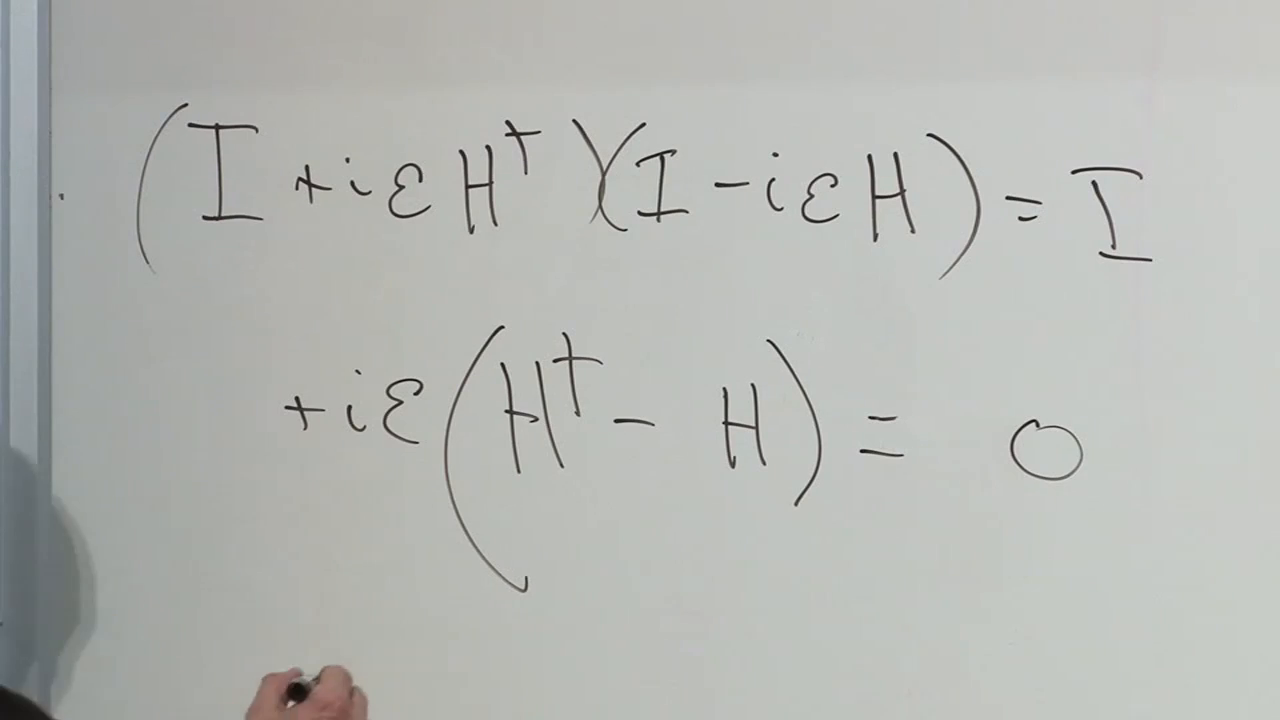
\includegraphics[width=0.86\textwidth]{lecture_04_figure_03.png}
\caption{一次のユニタリ性の計算により、微小生成子はエルミートでなければならないことが強制される。}
\lectureframe{00:43:38}
\end{figure}

文字\(H\)はエルミートを表すのではなく、\emph{ハミルトニアン}を表す。それがエルミートであるから、可観測量を表す。それはエネルギーと同一視され、より構造的には時間並進の生成子と同一視される。この同一視は名前で尽くされるものではない。既知の古典極限をもつ系では、量子的な\(H\)は古典的ハミルトニアンの力学を再現しなければならない。対称性、自由度、物理的判断、そして最終的には実験が、どのエルミート演算子が特定の系のハミルトニアンであるかを決める。

\begin{classroomqa}
\audiencequestion{任意のエルミート演算子を\(H\)に用いることができるのか。実際のものを選ぶのは何か。}
\lecturerresponse{ここまでの導出は、系のヒルベルト空間上の任意のエルミート演算子を許す。物理はその系の自由度から構成されるものを選ぶ。スピンに対しては、スピン演算子と外部場から構成されなければならない。対称性と既知の相互作用が可能性を狭め、実験が残りの定数、時には形そのものを確定する。}
\end{classroomqa}

ハミルトニアンは陽に時間に依存してもよい。電流を変化させている磁場が簡単な例を与える。外部パラメータが時間に依存しないならば、\(H\)は陽な時間依存性をもたない。これが時間並進不変性である。パラメータが時間的に駆動されるならば、エネルギーは保存される必要はない。

\begin{classroomqa}
\audiencequestion{短時間展開において、\(H\)は定数なのか、それとも\(H(0)\)とすべきなのか。}
\lecturerresponse{時間に依存しない問題では、\(H\)はどの時刻でも同じ演算子である。より一般には、時刻\(t\)から始まる局所的なステップには\(H(t)\)が含まれる。ここでの導出はまず時間並進不変な場合を扱い、後に陽な時間依存性がエネルギー保存をどう変えるかを述べる。}
\end{classroomqa}

\section{時間依存Schr\"odinger方程式}

式~\eqref{eq:l4-small-u}を状態に適用する：
\begin{equation}
\ket{\psi(\epsilon)}=(I-i\epsilon H)\ket{\psi(0)}+O(\epsilon^2).
\end{equation}
整理して\(\epsilon\)で割ると、
\begin{equation}
\frac{\ket{\psi(\epsilon)}-\ket{\psi(0)}}{\epsilon}
=-iH\ket{\psi(0)}+O(\epsilon).
\label{eq:l4-difference-quotient}
\end{equation}

\begin{figure}[htbp]
\centering
\includegraphics[width=0.86\textwidth]{lecture_04_figure_04.png}
\caption{微小な状態の更新を整理してベクトル値の差分商にしたもの。}
\lectureframe{00:51:42}
\end{figure}

ベクトルを微分することに特別な謎はない。二つのベクトルは引き算でき、その差は数で割ることができ、その極限が別のベクトルを定義する。上でゼロと呼んだ基準時刻は任意の瞬間でよい。したがって\(\epsilon\to0\)を取ると
\begin{equation}
\boxed{\frac{d}{dt}\ket{\psi(t)}=-iH\ket{\psi(t)}}
\qquad(\hbar=1).
\label{eq:l4-schrodinger-natural}
\end{equation}が得られる。

\begin{figure}[htbp]
\centering
\includegraphics[width=0.86\textwidth]{lecture_04_figure_05.png}
\caption{完成した板書の導出は、枠で囲まれた時間依存のSchr\"odinger方程式に到達する。}
\lectureframe{00:56:11}
\end{figure}

これは一般化された時間依存のSchr\"odinger方程式である。粒子の波動関数に対するおなじみの微分方程式は、この抽象的な状態ベクトル方程式の一つの表現である。これを使うには、\(H\)と初期状態を知らなければならない。

有限の区間に対しては、微分方程式を解く。\(H\)が時間に依存しないとき、微小なステップを繰り返し合成すると
\begin{equation}
U(t)=e^{-iHt}
\qquad(\hbar=1),
\end{equation}
が得られる。これはすべての小さなステップを合成することの正確な版である。時間に依存するハミルトニアンには時間順序が必要であり、その精密化は後回しにする。

\begin{classroomqa}
\audiencequestion{展開は微小な区間を用いた。長い時間の後の状態を決めるものは何か。}
\lecturerresponse{微小な更新を繰り返し適用するか、等価に微分方程式を解く。時間に依存しない\(H\)に対して、小さなステップの積は\(e^{-iHt/\hbar}\)になる。}
\end{classroomqa}

\subsection{プランク定数の復元}

前の方程式は\(\hbar=1\)とする単位を用いていた。次元解析は\(\hbar\)がどこに属するかを示す。導関数は時間の逆数の次元を持ち、一方\(H\)はエネルギーの次元を持つ。\(\hbar\)はエネルギー×時間の次元を持つので、
\begin{equation}
\boxed{i\hbar\frac{d}{dt}\ket{\psi(t)}=H\ket{\psi(t)}}.
\label{eq:l4-schrodinger}
\end{equation}
等価に、微小演算子は\(U(\epsilon)=I-i\epsilon H/\hbar+O(\epsilon^2)\)であり、有限の時間に依存しない発展は\(U(t)=e^{-iHt/\hbar}\)である。

\begin{classroomqa}
\audiencequestion{プランク定数は正確にどこに入るのか。}
\lecturerresponse{プランク定数は、等価な形のいずれかに入る。
\begin{align*}
i\hbar\,\partial_t\ket{\psi}&=H\ket{\psi},\\
\partial_t\ket{\psi}&=-\frac{i}{\hbar}H\ket{\psi}.
\end{align*}
\(\hbar\)はエネルギー×時間の単位を持つので、両者は次元が一致する。}
\end{classroomqa}

状態は式~\eqref{eq:l4-schrodinger}に従って決定論的に発展する。測定結果は、連続的に変化する状態からボルンの規則によってサンプリングされるため、依然として統計的である。

\begin{classroomqa}
\audiencequestion{導出は可逆性に依存するのか、また状態を乱す測定をどのようにして生き延びられるのか。}
\lecturerresponse{それは線形発展と内積の保存に依存する。この方程式は孤立系を支配する。測定装置は物理系の一部となるほど強く相互作用し、無視できない。合成系と装置は量子力学的に扱わなければならず、それらのエンタングルメントこそが、測定を分析する前に理解されなければならないものである。}
\end{classroomqa}

\section{期待値は平均を意味する}

量子力学のダイナミクスを古典方程式と比較するには、観測量の平均値が必要である。標準的な名称\emph{期待値}は誤解を招く可能性がある。\(+1\)と\(-1\)だけを取る公平な変数では、平均はゼロであるが、ゼロは決して観測されない。対称な分布では、平均の近傍全体でさえ消えることがある。平均、中央値、最頻値は、滑らかで単峰の分布では一致することがあるが、一般には一致しない。

\(L\)が値\(\lambda_i\)を確率\(P(\lambda_i)\)で返すことができるなら、
\begin{equation}
\overline{\lambda}=\sum_i\lambda_iP(\lambda_i).
\label{eq:l4-probability-average}
\end{equation}
と定義する。これは分布の一次モーメントであり、一回の試行の結果についての約束ではない。

\begin{classroomqa}
\audiencequestion{最も頻繁な値こそ期待すべきものではないのか。}
\lecturerresponse{最も頻繁な値は最頻値であり、重み付き平均は平均である。単純で狭い分布では一致することがあるが、二峰性の分布では平均が本質的に確率ゼロの領域にあることがある。期待値という言葉は数学的な平均を指し、必ずしも最も可能性の高い単一の結果を指すわけではない。}
\end{classroomqa}

繰り返し試行は数学的な平均をデータに結びつける。通常の独立性と有限モーメントの仮定の下で、大数の法則は標本平均の確率的収束を述べる。それらはすべての有限列が平均の近くにあることを保証しない。同一のスピン結果が異常に長く続くことは依然として可能であり、ただありそうにないだけである。これは、熱力学第二法則が例外のない微視的禁止則となることを妨げるのと同じ統計的な微妙さである。

\begin{classroomqa}
\audiencequestion{公正なスピン実験がたまたま百万回連続で上を与えたなら、その平均は本当に上なのか。}
\lecturerresponse{その特定の試行の標本平均は確かに上である。理論的期待値は依然としてゼロである。独立な試行の数が増えるにつれて、標本平均は高い確率で理論的平均に近づくが、確率論は例外的な有限列をすべて排除することは決してない。}
\end{classroomqa}

\subsection{演算子サンドイッチ}

規格化された状態を\(L\)の正規直交固有基底で展開する：
\begin{equation}
\ket{A}=\sum_i\alpha_i\ket{\lambda_i},
\qquad
\bra{A}=\sum_j\alpha_j^*\bra{\lambda_j}.
\end{equation}
ボルンの規則と式~\eqref{eq:l4-probability-average}より
\begin{equation}
\overline{\lambda}=\sum_i\lambda_i|\alpha_i|^2.
\end{equation}
ここで計算する
\begin{align}
\bra{A}L\ket{A}
&=\sum_{i,j}\alpha_j^*\alpha_i
  \bra{\lambda_j}L\ket{\lambda_i}\\
&=\sum_{i,j}\alpha_j^*\alpha_i\lambda_i
  \braket{\lambda_j}{\lambda_i}\\
&=\sum_i\lambda_i|\alpha_i|^2.
\end{align}
\(\braket{\lambda_j}{\lambda_i}=\delta_{ji}\)であるから、二重和は崩壊する。したがって
\begin{equation}
\boxed{\expect{L}_A=\bra{A}L\ket{A}}.
\label{eq:l4-expectation-sandwich}
\end{equation}

\begin{figure}[htbp]
\centering
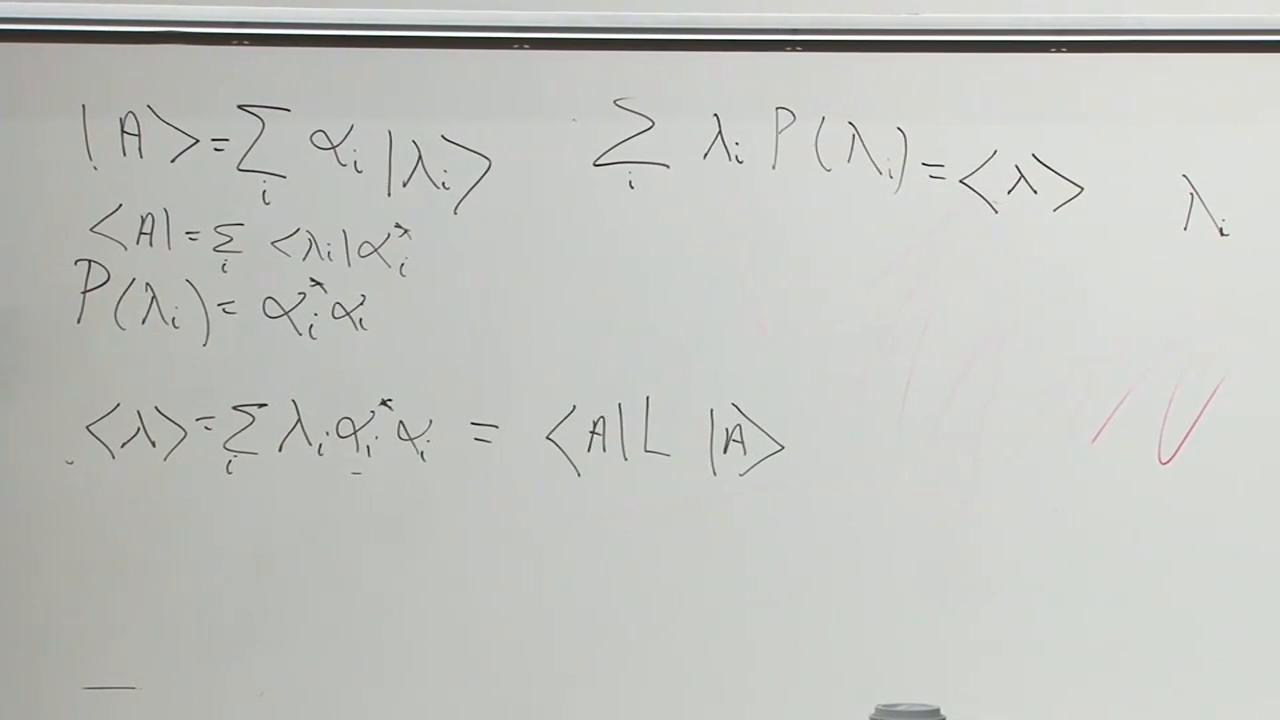
\includegraphics[width=0.86\textwidth]{lecture_04_figure_06.png}
\caption{固有基底展開は確率的平均を演算子サンドイッチ\(\bra{A}L\ket{A}\)に帰着させる。}
\lectureframe{01:11:50}
\end{figure}

平均には山括弧と上線の両方を用いる。状態が発展するとき、
\begin{equation}
\expect{L}_t=\bra{\psi(t)}L\ket{\psi(t)}.
\end{equation}
下付き添字は、状態、したがって平均が時間に依存することを思い出させるだけである。現在のSchr\"odinger描像の議論では、明示的な時間依存が述べられない限り、\(L\)自体は固定されている。

\begin{classroomqa}
\audiencequestion{\(t\)は括弧の外に書くべきか、また上線は標本平均を意味するのか。}
\lecturerresponse{どちらの記法も時間依存を示すように注釈を付けることができるが、標準的な量子記法は\(\expect{L}_t\)、あるいは\(\ket{\psi(t)}\)から時間が了解される単なる\(\expect{L}\)である。ここで上線は理論的確率平均、すなわち一次モーメント\(\sum_i\lambda_iP(\lambda_i)\)を表し、特に有限データの標本平均を表すものではない。}
\end{classroomqa}

\section{平均はどのように発展するか}

サンドイッチを積の法則で微分する：
\begin{equation}
\frac{d}{dt}\expect{L}
=
\left(\frac{d}{dt}\bra{\psi}\right)L\ket{\psi}
+
\bra{\psi}L\left(\frac{d}{dt}\ket{\psi}\right).
\label{eq:l4-product-derivative}
\end{equation}
\(\hbar=1\)単位では、ケット方程式とそのエルミート共役は
\begin{align}
\frac{d}{dt}\ket{\psi}&=-iH\ket{\psi},\\
\frac{d}{dt}\bra{\psi}&=+i\bra{\psi}H.
\end{align}
\(i\)の符号は複素共役で変わり、\(H^\dagger=H\)である。式~\eqref{eq:l4-product-derivative}への代入により
\begin{align}
\frac{d}{dt}\expect{L}
&=i\bra{\psi}HL\ket{\psi}
-i\bra{\psi}LH\ket{\psi}\\
&=i\bra{\psi}(HL-LH)\ket{\psi}.
\end{align}

演算子は可換である必要はない。それらの順序は行列の順序が重要であるのと同じように重要である。定義する
\begin{equation}
[H,L]=HL-LH.
\end{equation}
すると
\begin{equation}
\boxed{\frac{d}{dt}\expect{L}=i\expect{[H,L]}}
\qquad(\hbar=1).
\label{eq:l4-average-evolution-natural}
\end{equation}

\begin{figure}[htbp]
\centering
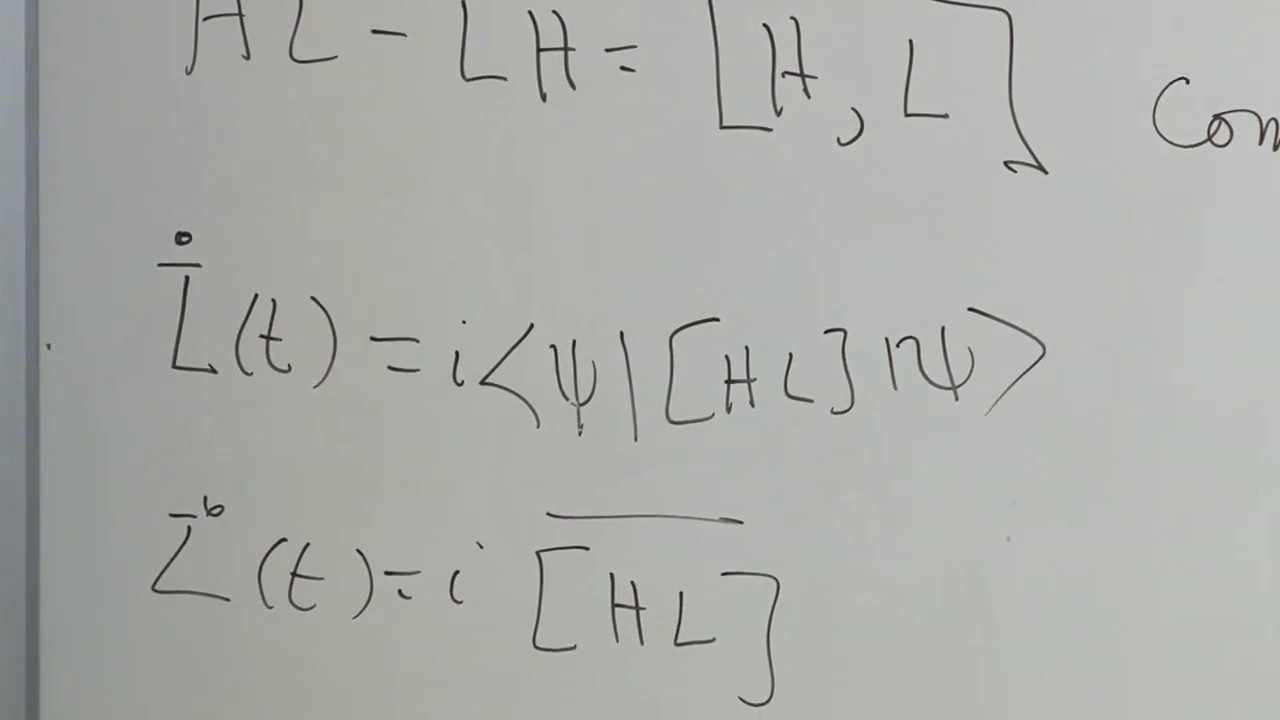
\includegraphics[width=0.86\textwidth]{lecture_04_figure_07.png}
\caption{平均の時間微分は交換子の期待値によって支配される。}
\lectureframe{01:22:22}
\end{figure}

次元を復元すると、
\begin{equation}
\boxed{\frac{d}{dt}\expect{L}
=\frac{i}{\hbar}\expect{[H,L]}
=-\frac{i}{\hbar}\expect{[L,H]}}.
\label{eq:l4-average-evolution}
\end{equation}
\(L\)自体が明示的に時間に依存するなら、一般方程式は追加項\(\expect{\partial L/\partial t}\)を含む。ここで\(L\)は固定されている。

\begin{classroomqa}
\audiencequestion{交換子方程式の符号は本当にプラス\(i\)か。}
\lecturerresponse{はい、\([H,L]=HL-LH\)とすると、結果は\(+(i/\hbar)\expect{[H,L]}\)である。交換子を逆にするとその符号が逆になり、等価な形\(-(i/\hbar)\expect{[L,H]}\)を与える。}
\end{classroomqa}

\begin{classroomqa}
\audiencequestion{ブラ方程式は複素共役によって得られたのか、それともエルミート共役によって得られたのか、そしてなぜ微分は左に残るのか。}
\lecturerresponse{それはエルミート共役である。ケットの微分はケットであり、その微分の双対は対応するブラの微分である。これは差分商から直接見ることができる：ブラの差はブラであり、ちょうどケットの差がケットであるのと同じである。ここで時間はパラメータであり、順序を逆にしなければならない演算子ではない。}
\end{classroomqa}

\section{古典的影}

古典ハミルトン力学では、明示的な時間依存をもたない位相空間関数\(L(q,p)\)は次を満たす
\begin{equation}
\frac{dL}{dt}=\{L,H\}_{\mathrm{PB}},
\label{eq:l4-poisson-evolution}
\end{equation}
ここで\(\{\cdot,\cdot\}_{\mathrm{PB}}\)はポアソン括弧である。これを式~\eqref{eq:l4-average-evolution}と比較せよ。両方の括弧は反対称である：
\begin{align}
\{L,H\}_{\mathrm{PB}}&=-\{H,L\}_{\mathrm{PB}},\\
[L,H]&=-[H,L].
\end{align}
また両方とも積に対して微分として作用する：
\begin{align}
\{LM,H\}_{\mathrm{PB}}
&=\{L,H\}_{\mathrm{PB}}M+L\{M,H\}_{\mathrm{PB}},\\
[LM,H]
&=L[M,H]+[L,H]M.
\label{eq:l4-commutator-product}
\end{align}
交換子の恒等式は\(LHM\)を加えたり引いたりすることで従う：
\begin{align}
LMH-HLM
&=(LMH-LHM)\\
&\quad +(LHM-HLM)\\
&=L(MH-HM)\\
&\quad +(LH-HL)M.
\end{align}

この類似は対応関係を示唆する
\begin{equation}
[A,B]
\quad\longleftrightarrow\quad
i\hbar\{A,B\}_{\mathrm{PB}},
\label{eq:l4-dirac-correspondence}
\end{equation}
あるいは等価に
\begin{equation}
\{A,B\}_{\mathrm{PB}}
\quad\longleftrightarrow\quad
-\frac{i}{\hbar}[A,B].
\end{equation}

\begin{figure}[htbp]
\centering
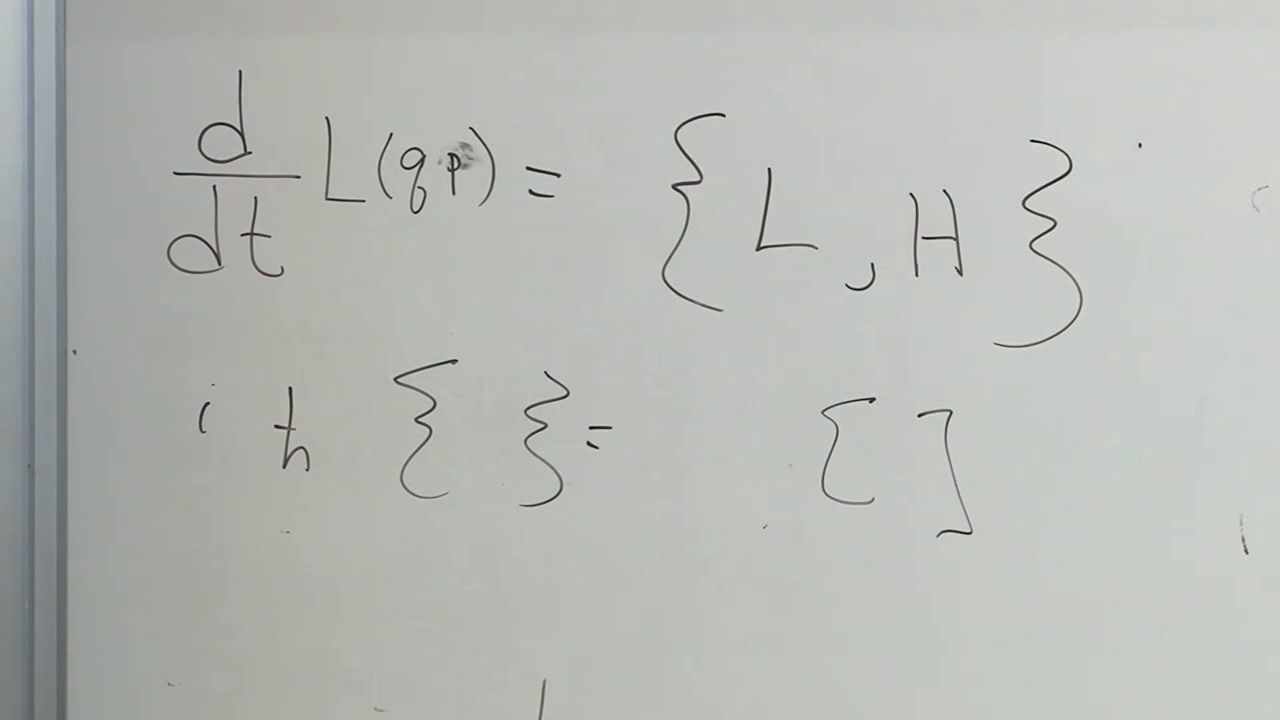
\includegraphics[width=0.86\textwidth]{lecture_04_figure_08.png}
\caption{古典的ポアソン括弧方程式と量子交換子対応、\(\hbar\)を復元したもの。}
\lectureframe{01:32:32}
\end{figure}

ディラックはこの関連を認識し、量子力学への道として用いた。それでもなお、これは普遍的な置換規則ではなく対応関係として扱わなければならない：演算子順序の曖昧さが現れることがあり、古典極限は量子力学から導出されなければならない。概念的には、量子力学が第一であり、古典力学は適切な状態とスケールに対するその近似である。歴史的類推が関係の発見に役立つとはいえ、交換子がポアソン括弧に先行する。

\begin{classroomqa}
\audiencequestion{なぜ\(H\)をエネルギーと呼び、対称性原理を課す前にエネルギー保存を推論するのか。}
\lecturerresponse{この段階では、\(H\)は時間並進のエルミート生成子であることが厳密に成り立っている。それをエネルギーと呼ぶことは物理的な同定であり、古典極限が知られているところで確認されなければならない。適切な状態にある大きな系や重い系では、量子平均は古典方程式に従わなければならず、量子的な\(H\)は古典的ハミルトニアンに接続しなければならない。以下の保存の主張は、この生成子が時間に陽に依存しないことを仮定している。}
\end{classroomqa}

\section{平均エネルギーは保存される}

時間に依存しないハミルトニアンのもとで、式~\eqref{eq:l4-average-evolution}において\(L=H\)とおく。
\begin{equation}
\frac{d}{dt}\expect{H}
=\frac{i}{\hbar}\expect{[H,H]}.
\end{equation}
すべての演算子はそれ自身と可換であり、
\begin{equation}
[H,H]=HH-HH=0,
\end{equation}
したがって
\begin{equation}
\boxed{\frac{d}{dt}\expect{H}=0}.
\label{eq:l4-energy-conservation}
\end{equation}

\begin{figure}[htbp]
\centering
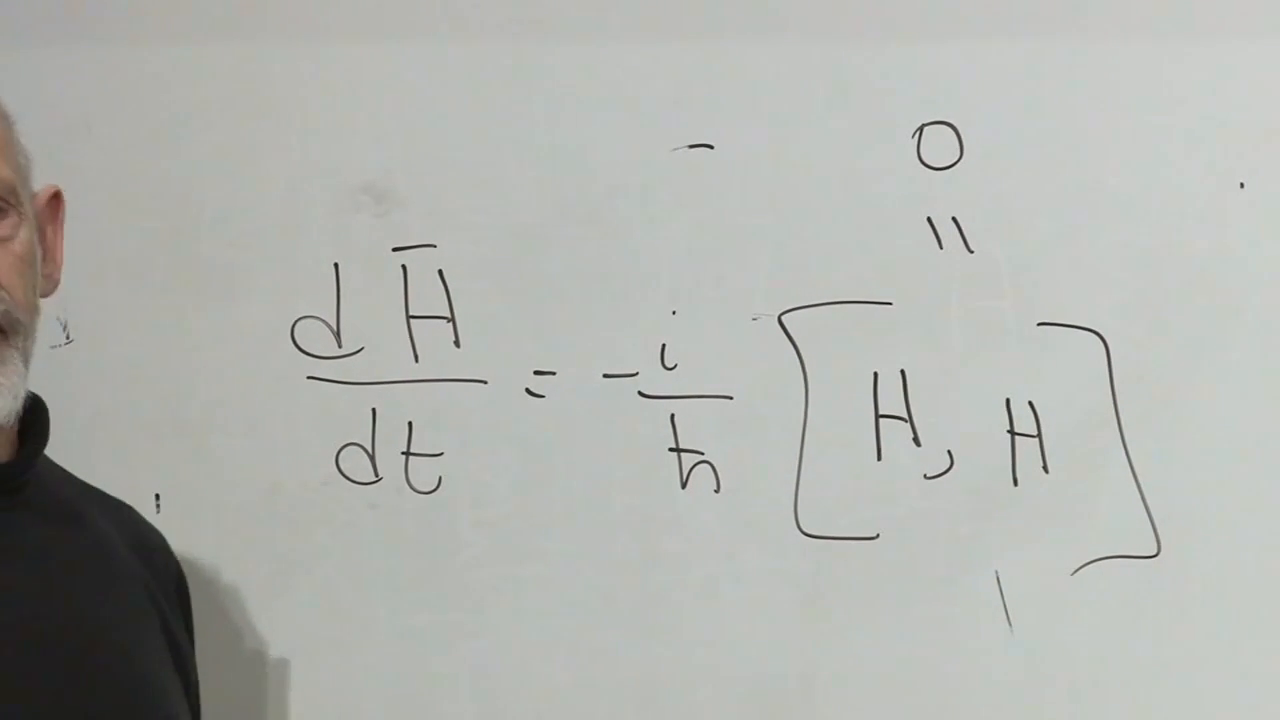
\includegraphics[width=0.86\textwidth]{lecture_04_figure_09.png}
\caption{ハミルトニアンがそれ自身と可換であるため、平均エネルギーの保存は直ちに従う。}
\lectureframe{01:39:30}
\end{figure}

これは、意図的に控えめな主張を証明している。すなわち、平均エネルギーは一定である。エネルギー分布全体に関するより強い主張は、同じ力学から従うであろう。もし\(H\)が時間に陽に依存するならば、余分な陽の微分は消える必要はなく、駆動された系はそのパラメータを変化させるものとの間でエネルギーを交換しうる。

二つの糸口が未解決のまま残っている。任意軸のスピン確率の計算は依然として待たれており、状態更新の問題はまだ導出されていない。介入と介入の間、孤立した状態はユニタリに発展する。測定の間、系と装置は相互作用し、もつれ合う。

\begin{classroomqa}
\audiencequestion{任意軸に沿って測定されたスピンについて約束された確率はどうなったのか。}
\lecturerresponse{一般的な力学が利用可能な時間を費やした。スピンの計算は次の具体的な応用として残っており、この構造的枠組みの後に再開される。}
\end{classroomqa}

\begin{classroomqa}
\audiencequestion{収縮の公準なしに、どうして公準が完全でありうるのか。}
\lecturerresponse{今のところ、収縮は暫定的な言葉である。測定は系と装置の間にもつれを確立する。複合系ともつれが展開されるまでは、測定過程を正直にモデル化することはできない。それが次の概念的段階である。}
\end{classroomqa}
